% !TEX root = ../thesis.tex
\chapter{Progenitor search in SN 1006}
\label{chap:sn1006}


\section{Introduction}

The search for a donor star in \sn{1572}{}\ has not turned up an obvious candidate. However, we have detected two objects (\starb\ and \starg) exhibiting some unusual properties, which while interesting, ultimately seem inconsistent with the expectations of any viable donor star scenario. \Gls{donor} star scenarios are theoretical in their nature and any actual donor star is likely to not exhibit all features predicted by the model. Therefore, we have reached an impasse with \sn{1572}{} and more detailed observations will likely not provide a definitive answer if either of these two stars were involved in the progenitor system. An obvious way forward is to scrutinise stars in other \snia\ remnants and see if any of those have similar properties to \starb\ or \starg. The remnant of \sn{1006}{} is the ideal object for this kind of follow-up search. 

The lack of a central neutron star, observation of several tenths of a solar mass of iron inside the remnant \citep{1997ApJ...481..838H} and the the high peak luminosity and basic light curve shape \citep[visible for several years][]{1965AJ.....70..748G} all indicate that \sn{1006}{} was a \snia. The remnant has a secure distance, measured by \citet{2003ApJ...585..324W}, who combined the proper motion and the radial velocity of the expanding shell to measure the distance to 2.2~\kpc, making \sn{1006}{} the closest of the ancient \snia\ remnants (consistent \sn{1006}{} being the brightest).   The geometric centre of the remnant is well determined from both \xray\ and radio observations \citep{2003ApJ...585..324W}. In addition, the interior of the remnant has been probed with UV background sources \citep{2005ApJ...624..189W}. 

This revealed the aforementioned iron core as well as a silicon-rich shell. The remnant has been searched for possible objects associated with the supernova explosion previously, and an unusual O-star had been identified as a possible donor star to \sn{1006}{}. This unusual O-Star was identified near the centre of \sn{1006}{} by \citet{1980ApJ...241.1039S} and is now called Schweizer-Middleditch Star (\smstar). After successful identifications of neutron stars in both the Vela Remnant and the Crab Remnant this was thought to be the third identification of a stellar remnant in a historical supernova. Subsequent UV spectroscopic follow-up of the \smstar\ by \citet{1983ApJ...269L...5W}, showed strong \ion{Fe}{2} lines with a profile broadened by a few thousand \kms. In addition, \citet{1983ApJ...269L...5W} identified redshifted \ion{Si}{2}, \ion{Si}{3} and \ion{Si}{4} lines. Their conclusion was that these absorption lines stem from the remnant and place the \smstar\ behind the remnant, making it unrelated to \sn{1006}{}. Although unrelated, the \smstar\ is an ideal object to probe the remnant and measure upper limits for interstellar extinction \citep[E(B-V) = 0.1][]{1993ApJ...416..247W,2003ApJ...585..324W}.


SN 1006 has several properties which make it well suited to undertake a progenitor search.  Although the remnant is the oldest among the known \snia\ remnants, its age is still young enough that  the remnant's centre is well determined, and the motion of any potential donor star low enough that only a small area of stars need to be searched. Furthermore, this elapse of 1005 years is a short length of time relative to the timescales of stellar evolution for donor stars \cite[see][]{2000ApJS..128..615M} - we still expect a potential donor star to be close to the same state as directly after the supernova explosion. In addition, \sn{1006}{} has a low interstellar extinction, which eases the determination of stellar parameters. These serendipitous conditions for the \sn{1006}{} remnant led us to launch a photometric and spectroscopic campaign to search for the donor star. Our photometric observations were taken at Siding Spring Observatory with the 2.3m Telescope imager. The spectroscopic observations were undertaken with the high resolution multi-object spectrograph \gls{flames} attached to the \gls{vlt}.


In Section \ref{sec:obs_red} we outline the observations as well as data reduction of the photometric and spectroscopic data. Section \ref{sec:sn1006_analysis} is split into four subsections, namely radial velocity, stellar rotation and stellar parameters. We conclude this chapter in Section \ref{sec:sn1006:conclusion} and discuss the possible implications of our initial find as well as outlining some future work.


\section{Observations and Data Reduction}
\label{sec:obs_red}
\subsection{Photometric Observations}
\Gls{ccd} images of \sn{1006}{} were obtained using the imaging camera at the Nasmyth-B focus of the ANU 2.3~m Telescope at
the Siding Spring Observatory, on 11 May 2004. We exposed for 1860~s in U-Band, 1490~s in B-Band, 788~s in V-Band and 1860~s in I-Band. For calibration purposes we took images of the PG1633 and PG1047 standard star regions in the same filters. The seeing ranged between 1\arcsec and 2\arcsec, and the conditions were photometric. 
The data were bias corrected and flatfielded (using skyflats) using \gls{pyraf}.

For our photometric data reduction we fitted an astrometric solution using astrometry from the \twomass\ point source catalogue \citep{2006AJ....131.1163S} to our frames. 
We used \gls{sextractor} to measure the magnitudes of the objects in the frames and then calibrated our photometry to a standard Bessell Filter system using the Stetson magnitudes \footnote{This research used the facilities of the Canadian Astronomy Data Centre operated by the National Research Council of Canada with the support of the Canadian Space Agency} of our standard fields PG1633 and PG1047 .  

The measured magnitudes were supplemented with near infrared magnitudes from the \twomass\ point source catalogue (see Table \ref{tab:sn1006_twomass} and \ref{tab:sn1006_photometry} ). Subsequently we checked the photometric measurements, by plotting the obtained $B-V$ colours against the $V-K$ colours (see Figure \ref{fig:colour_check}).
\begin{figure}[htbp] %  figure placement: here, top, bottom, or page
   \centering
   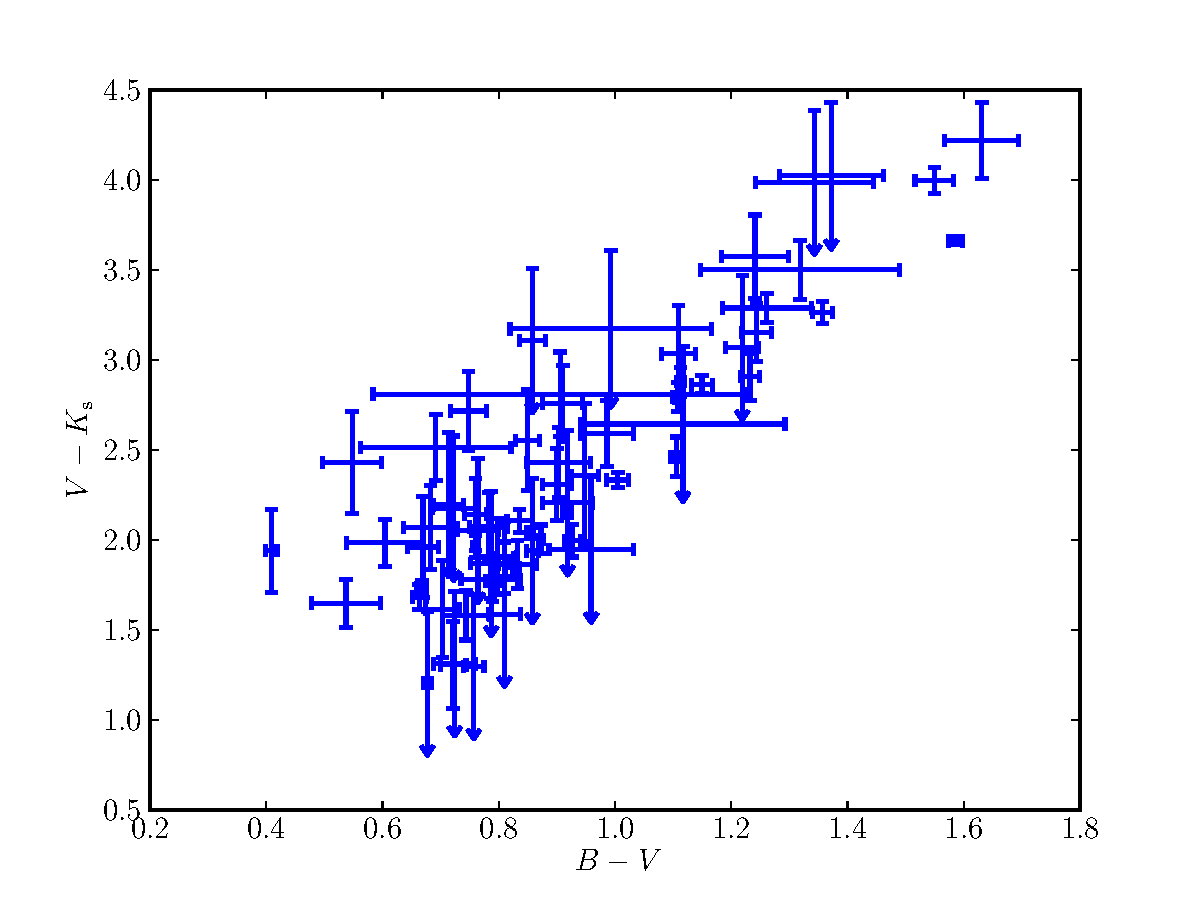
\includegraphics[width=\textwidth]{chapter_sn1006/plots/color_bv_vk.pdf} 
   \caption[Colour-colour plot of all candidates in SN 1006 to check photometry]{Colour-colour plot of all candidates in SN 1006 to check photometry. The correspondence is as expected given the uncertainties in the measurements.}
   \label{fig:colour_check}
\end{figure}

We have also computed temperatures from photometric colours by using the polynomials given in \citet{2010A&A...512A..54C}. In the first instance, we assumed a solar \gls{feh} for all stars, but the choice of \gls{feh} only has a minor influence on the temperature calculation (e.g. change of 300K between \feh=0 and \feh=-1) for the temperature. In addition, the temperature polynomial coefficients incorporating the metallicity are particularly small for the $V-K$ colour. All temperatures are listed in the optical photometry Table \ref{tab:sn1006_photometry} and infrared photometry Table \ref{tab:sn1006_twomass}.


\subsection{Spectroscopic Observations}

For the spectroscopy survey we used the \gls{vlt} instrument \gls{flames}, which can provide high resolution (R=25,000) optical spectra over a 25\arcmin\ field of view for up to 130 objects. In this mode, the spectral coverage is limited to 200~\AA, and we chose the wavelength region from 5139~\AA\ to 5356~\AA\ which contains the gravity sensitive \gls{mgb} Triplet as well as many iron lines to accurately measure metallicity. For the centre of our spectroscopic survey we chose the mean of the \xray\ and radio centre \citep[\rasc{15}{02}{22}{1}\ \decl{-42}{05}{49};][]{2003ApJ...585..324W}. We chose a search radius of 120\arcsec\ - corresponding to the motion of a star travelling 1250~\kms at 2.2~\kpc\ over 1000 years. This generous choice, which is more than four times our maximum expected escape velocity (see Figure \vref{fig:han2008_vrad}), was made to accommodate any errors in the choice of the centre. Although the models predict the surviving companion to be several hundred \lsun\ \citep{2000ApJS..128..615M}, we chose a limiting magnitude of $V=17.5$ ($0.5~\lsun(V)$ at 2.2~\kpc\ including extinction of E(B-V)=0.1) to accommodate a wide range of potential \gls{donor} stars. An exposure time of 3.8~hours was chosen to obtain spectra with high enough quality to measure rotation and basic stellar parameters (\snratio\ $>20$). For completeness and to not waste fibres we chose additional stars down to a magnitude limit of $V=19$, which are only used for radial velocity measurements. These constraints yielded 26 stars with $V<17.5~\textrm{mag}$ and 53 stars in the bin between $17.5<V<19~\textrm{mag}$ (for a total of 79 stars) for our survey (see Figure \ref{fig:overview_sn1006}). With fibre buttons not being able to be placed less than 11\arcsec\ apart, we had to split our candidates over three different setups. The first two setups were observed five times with 2775~seconds each. We deliberately chose bright stars for the last setup so that it only had to be observed three times with 2775 s each. In addition, we placed spare fibres on three bright stars (R$\approx 10$; 2MASS J15032744-4204463, 2MASS J15031746-4204165, 2MASS J15033195-4202356) located close to the edge of the 25\arcmin\ field of view for calibration purposes. Additional spare fibres were placed on sky positions, which were chosen to be far from \twomass\ sources and manually inspected on DSS images to be in star free regions.
\begin{figure}[tb] %  figure placement: here, top, bottom, or page
   \centering
   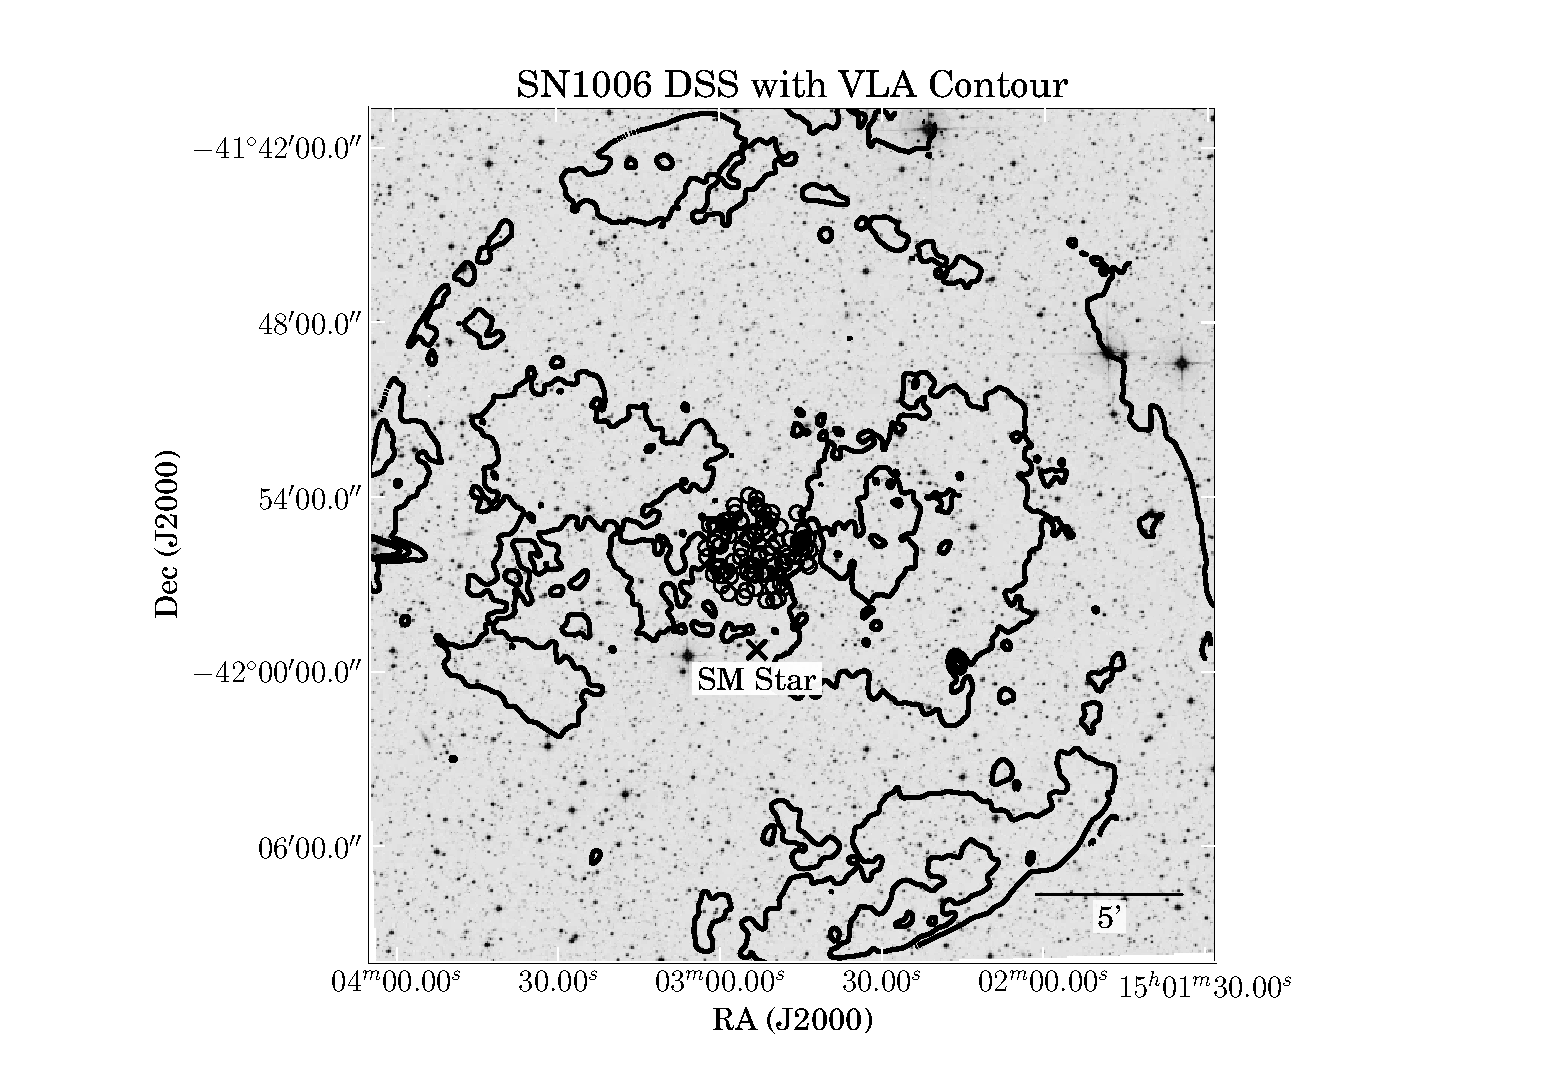
\includegraphics[width=\textwidth, trim=2cm 0 4cm 0, clip]{chapter_sn1006/plots/sn1006_overlay_withsm.pdf} 
   \caption[Overview of candidates and remnantin SN 1006]{Optical DSS image with radio contour overlay (VLA). The black circles in the centre show the 79 program stars. Additionally we have marked the `spurious` donor the \smstar.}
   \label{fig:overview_sn1006}
\end{figure}
In addition, to our night time calibration, which included simultaneous arc exposures with four fibres for each observation block, we received standard daytime calibrations. In total, 13 observation blocks with an exposure time of 2775~seconds each were obtained. Table \ref{tab:observations} provides the Observing ID, modified julian date, mean seeing, mean airmass, setup name and heliocentric correction for all observations (all data is available under ESO Program ID: 083.D-0805(A)). Due to broken fibres, not all stars where observed for the expected length of time. Broken fibres caused \candstar{31} not to be observed at all in this project (see Figure \ref{fig:sn1006:zoomed_overview}) - although a $V=17.87~\textrm{mag}$ is not part of our primary sample.
\begin{deluxetable}{cccccc}
\tablecaption{Observations}
\tablehead{\colhead{ObsID} & \colhead{MJD} & \colhead{FWHM} & \colhead{Airmass} & \colhead{SetupName} & \colhead{$\Delta v_{\rm helio}$}\\ 
\colhead{-} & \colhead{d} & \colhead{\arcsec} & \colhead{-} & \colhead{-} & \colhead{\kms}}


\startdata
360737 & 54965.1 & 1.2 & 1.2 & SN1006 1 & 1.5\\
360739 & 54965.1 & 1.2 & 1.1 & SN1006 1 & 1.5\\
360740 & 54965.1 & 1.0 & 1.1 & SN1006 1 & 1.4\\
360741 & 54985.0 & 0.7 & 1.4 & SN1006 1 & -7.4\\
360742 & 54964.2 & 1.5 & 1.1 & SN1006 1 & 1.7\\
360743 & 54985.0 & 0.8 & 1.2 & SN1006 2 & -7.5\\
360745 & 54985.0 & 0.9 & 1.1 & SN1006 2 & -7.6\\
360746 & 54985.1 & 1.0 & 1.1 & SN1006 2 & -7.7\\
360747 & 54985.1 & 1.0 & 1.1 & SN1006 2 & -7.7\\
360748 & 54985.2 & 0.9 & 1.1 & SN1006 2 & -7.8\\
360749 & 54963.1 & 1.2 & 1.2 & SN1006 3 & 2.4\\
360751 & 54963.1 & 1.1 & 1.1 & SN1006 3 & 2.3\\
360752 & 54963.2 & 1.1 & 1.1 & SN1006 3 & 2.3\\
\enddata
\label{tab:observations}
\end{deluxetable}


\begin{figure}[tb] %  figure placement: here, top, bottom, or page
   \centering
   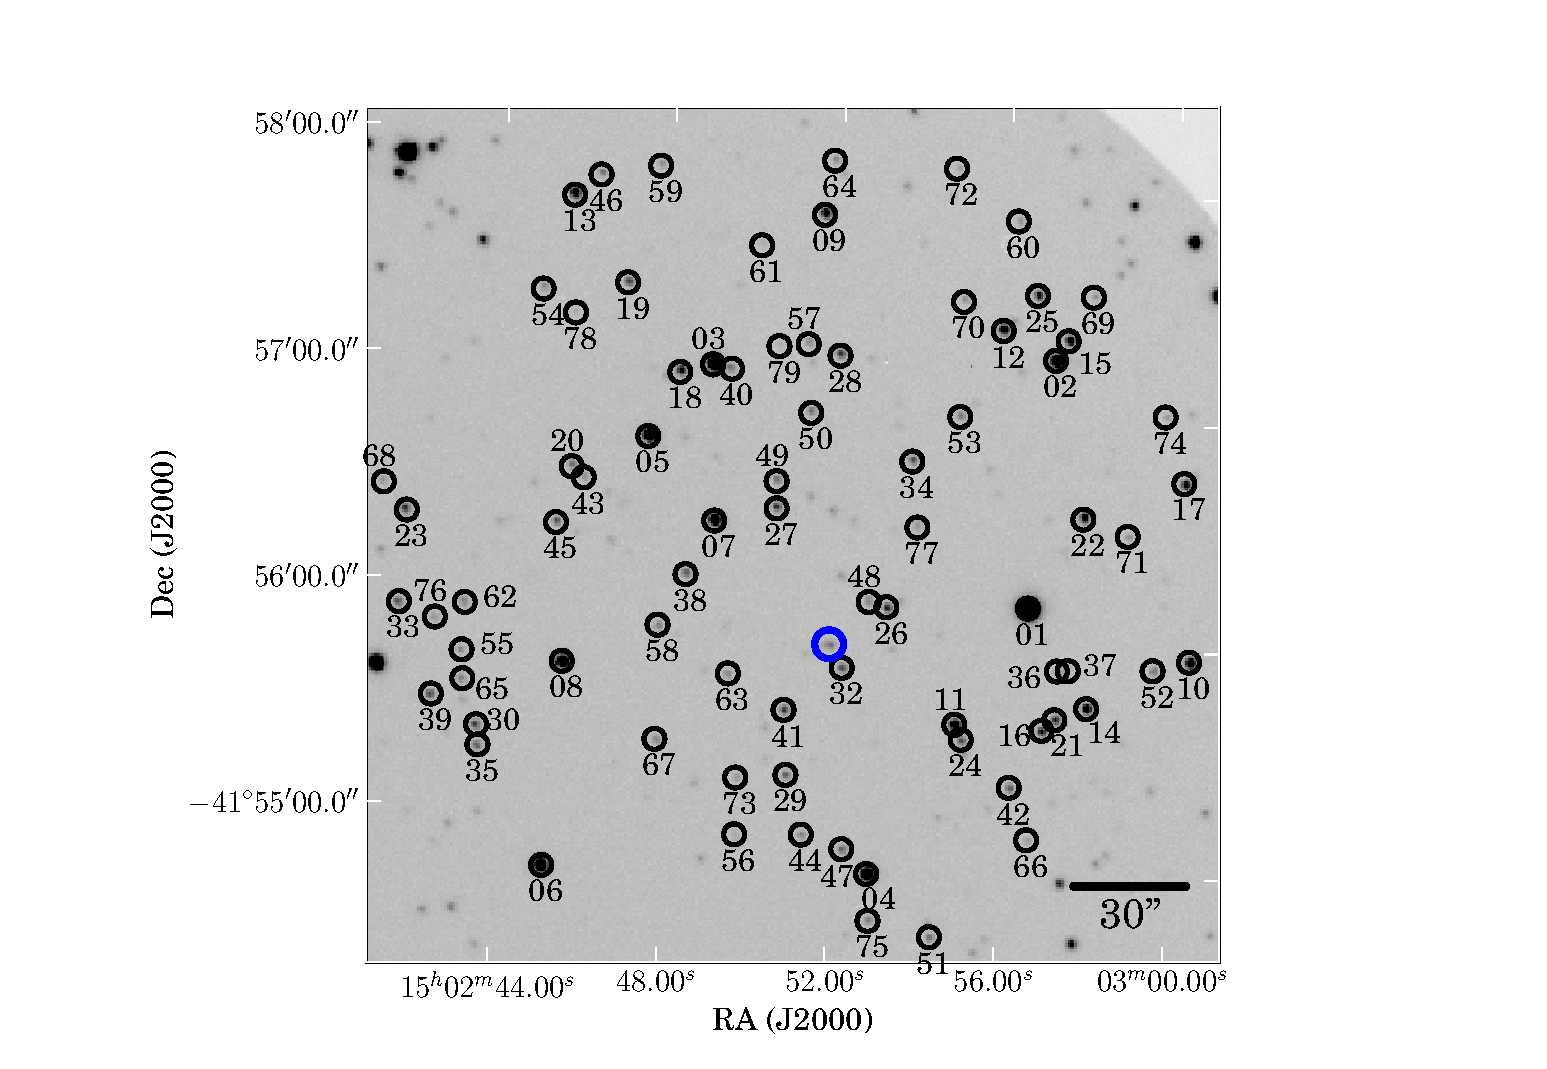
\includegraphics[width=\textwidth, trim=2cm 0 5cm 0, clip]{chapter_sn1006/plots/overview_labeled_sn1006.pdf} 
   \caption[Close-up of the candidates in SN 1006] {V-Band image taken by the 2.3~m Telescope. We have marked \candstar{31}, which was not observed due to broken fibres, with a blue circle. With the a brightness of $V=17.87$ \candstar{31} is fainter than our primary catalog ($V<17.5$~mag), and is the only star which lacks a spectrum to $V=19~\textrm{mag}$ in the remnant's centre.}
   \label{fig:sn1006:zoomed_overview}
\end{figure}


We first applied a cosmic ray removal tool on the raw 2D frames \citep{2001PASP..113.1420V}. The data was then reduced with the ESO-CPL pipeline (version 5.2.0), using the GIRAFFE instrument recipes (version 2.8.9). The only variation that was made to the default parameters was the usage of the Horne extraction algorithm instead of the "Optimal"-extraction algorithm. This yielded 366 individual spectra of the candidate stars and an additional 39 calibration star spectra. 


\section{Analysis}
\label{sec:sn1006_analysis}
\subsection{Radial Velocity}

\begin{figure}[tb] %  figure placement: here, top, bottom, or page
   \centering
   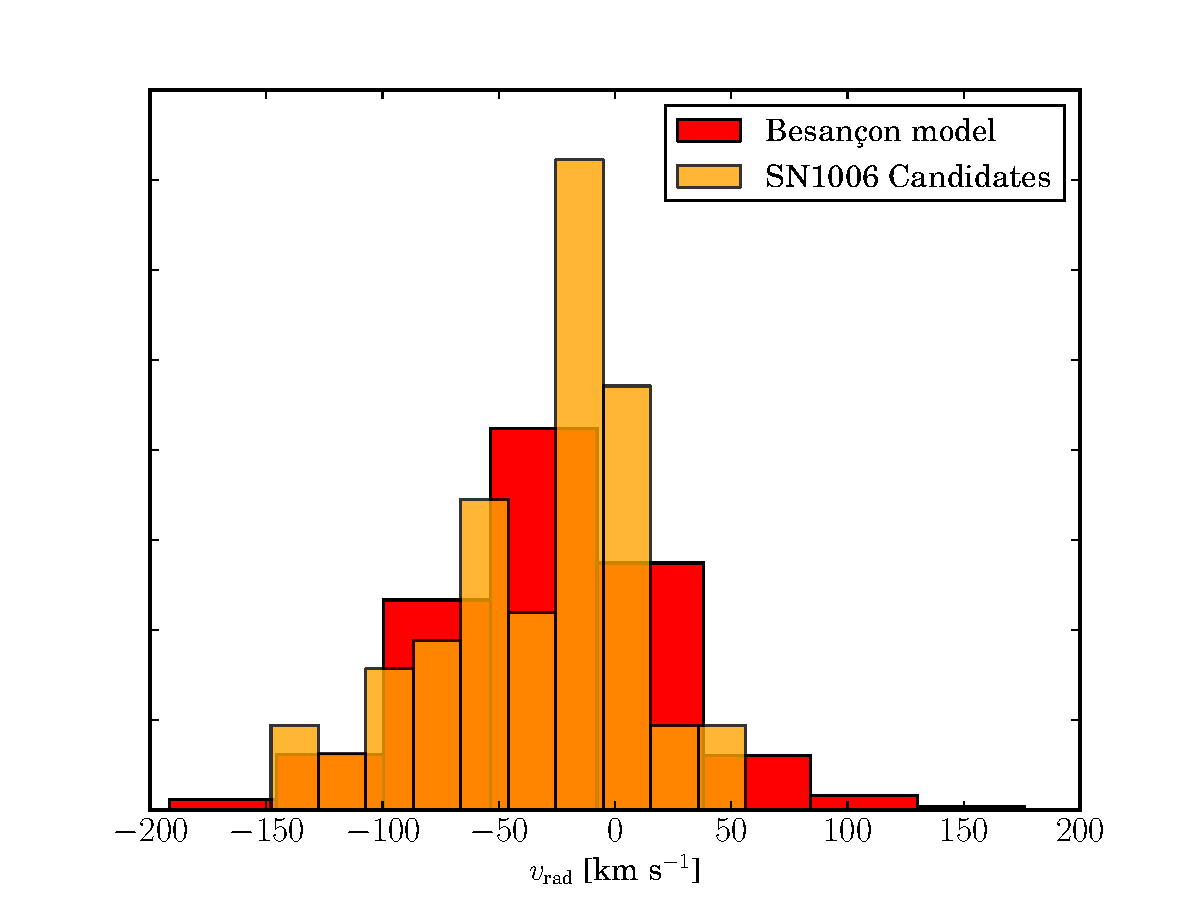
\includegraphics[width=\textwidth]{chapter_sn1006/plots/sn1006_vrad_besancon.pdf} 
   \caption[Radial velocity of all candidates in SN 1006 compared with Besan\c{c}on Model]{Comparison of all candidate stars with the distribution of stars taken from the the Besan\c{c}on kinematic model. The model input parameters were a search area of 1 square degree around the centre of \sn{1006}{} and a magnitude limit of $10<\textrm{V}<17.5$}
   \label{fig:sn1006_vrad_comp}
\end{figure}


To obtain radial velocities we employ a two step process. We used a solar spectrum from \citet{1984sfat.book.....K} with the standard cross-correlation technique described in \citet{1979AJ.....84.1511T} and implemented in the \gls{pyraf} task \textsc{fxcor}. The cross-correlation was performed on each individual spectrum. The results were then heliocentrically corrected, and then averaged for each star with a sigma clipping algorithm (see Table \ref{tab:sn1006_kinem}). We note that especially for faint objects we observe a second cross-correlation peak at 0~\kms and believe that this is reflected sun light from the moon. We believe that this has a negligible effect on our radial velocity measurement.
In Figure \ref{fig:sn1006_vrad_comp} we have compared our radial velocity measurements with the Besan\c{c}on kinematic model of the Milky way \citep{2003A&A...409..523R}. Our selection criteria for creating the  Besan\c{c}on kinematic model was all stars within 1 square degree of \sn{1006}{} and a magnitude cut of $10<\textrm{V}<17.5$. We compared the resulting 10000 stars to our 78 stars in the sample in Figure \ref{fig:sn1006_vrad_comp}. 




\subsection{Rotational Velocity}
\label{sec:sn1006_rotvel}
Due to the direction looked through the Galaxy, there is a large velocity spread in the direction of \sn{1006}{} (see Figure \ref{fig:sn1006_vrad_comp}) making it hard to isolate a \gls{donor} star based just on kinematic features. A distinguishing feature for a \gls{donor} star should be rotation (discussed in Chapter \ref{chap:sn1572_starg}), especially if the donor star isn't a giant. The rotational velocities in Chapters \ref{chap:sn1572_starg} \& \ref{chap:sn1572_hires} were all measured manually. In these previous measurements we selected weak iron lines and stacked them to obtain a line profile, which was compared to synthetically rotationally broadened lines. This was a feasible way for six spectra, it is however not feasible for more than 200 spectra. 

Measuring repetitive structures like line profiles is much more straight forward in Fourier space. The intrinsic spectrum ($f_\textrm{spectrum}$) of a star is broadened by a convolution of the intrinsic spectrum with a rotational broadening kernel ($g_\textrm{rotation}$). The next broadening is introduced by the instrument (instrumental kernel $h_\textrm{instrument}$) before being recorded on the detector. Assuming an unbroadened synthetic spectrum ($f_\textrm{synthetic}$), matching the intrinsic stellar spectrum, we can describe a convolution in Fourier space as,
\begin{align*}
	f_\textrm{observed} =& f_\textrm{spectrum} \otimes \underbrace{g_\textrm{rotation} \otimes h_\textrm{instrument}}_{f_\textrm{profile}}\\
     F(f_\textrm{spectrum} \otimes g_\textrm{rotation} \otimes h_\textrm{instrument}) =& F(f_\textrm{spectrum}) \times F(g_\textrm{rotation}) \times F(h_\textrm{instrument})\\
     \Rightarrow \frac{F(f_\textrm{observed})}{F(f_\textrm{synthetic})} \approx& F(f_\textrm{profile}),
\end{align*}
where $F$ denotes the Fourier transform. This yields the line profile which we can separate, knowing the resolution of the instrument, into an instrumental profile and a rotational kernel . This technique has been described by a selection of authors \citep[e.g.][]{1977ApJ...211..198G}. \textsc{fxcor} uses this technique to measure radial velocities from shift of the profile peak relative to rest. We have applied this technique successfully to extract the rotation for some of the stars were the quality of the spectra was adequate (see Table \ref{tab:sn1006_kinem}).


\subsection{Stellar Parameters}
\label{sec:sn1006_stelparam}

We obtained detailed stellar parameters for the donor candidates with $V<17.5$ by employing a grid based technique (three dimensional grid in \teff, \logg\ and \feh). \gls{moog} was used to synthesise the spectral grid using the model stellar atmospheres by \citet{2003IAUS..210P.A20C}. Line wings were taken into account up to 8~\AA\ away from line centre, which seemed to be a reasonable compromise between grid creation time and accuracy. For the atomic lines we merged values from the \gls{vald} with adjusted values (to reproduce the Arcturus and the Sun) from \cite{2008A&A...486..951G}. In addition, we used the measured molecular lines described in  \citet{1995KurCD..23.....K}. The final grid extends from 3500~K to 7500~K in \gls{teff} with a step size of 250~K, in \gls{logg} it ranges from  0 to 5 with a stepsize of 0.5 and in \feh\ it ranges from -2.5 to 0.5 with a stepsize of 0.5 (with an extra set of points at 0.2). 

We used the appropriate sections from the Solar spectrum \citep{1984sfat.book.....K} and the Arcturus spectrum \citep{2000vnia.book.....H} to calibrate our spectral grid. We measured stellar parameters by first finding the best fitting grid point and then using the minimizer \gls{minuit} to find a minimum by interpolating between the gridpoints \citep[described in Appendix \ref{chap:ndinterp} of this thesis;][]{Barber96thequickhull}. For the Sun we obtain stellar parameters of \teff=5825~K, \logg=4.4 and \feh=-0.12 and for Arcturus we obtain stellar parameters of \teff=4336~K, \logg=1.9, \feh=-0.67. We acknowledge the error in measurement, but believe our spectral grid to be accurate enough for distinguishing a potential donor candidate against an unrelated star. 

To measure our observed spectra we first fitted the continuum with Legendre polynomials with a maximum order of 3 and a sigma clipping algorithm discarding the lines. The order that gave the lowest \gls{rms} of the fit was used. We then combined the spectra using the previously measured \gls{vrad} and the computed heliocentric correction. In addition, we broadened the synthetic spectral grid with a rotational kernel for each star where applicable. These spectra were then fitedt using the previously described algorithm, except that we added the $B-V$ photometric temperature as a prior. As the photometric temperature uses the metallicity as an input parameter we recalculated the photometric temperature prior using the metallicity determined by the fit. This procedure was repeated until the gravity estimate converged to less than 0.1~dex. We believe our temperatures to be good to a few hundred K, our surface gravities as well as metallicities have a systematic uncertainty of roughly 0.5~dex. 

The stellar parameters can be seen, as fits to the spectra, in Figure \ref{fig:sn1006_candfit} and in tabulated form in Table \ref{tab:sn1006_stel_param}. The final set of stellar parameters shows a typical distribution of many dwarfs and a few giants. None of the stars seem to be unusual in any way. Giant stars, which are expected to have relatively low \vrot\ post explosion (but still $> 20~\kms$), are absent from the remnant's centre. 
%!TEX root = ../../thesis.tex
\ctable[
caption=SN 1006 candidates ($V<17.5$) stellar parameters,
label={tab:sn1006_stel_param},
width=\textwidth
]
{lXXXXX}{}{\FL
Name & $\teff $ & $\logg$ & \feh & 
V&\vrot \\ 
 & K & dex & dex& mag&\kms \ML
01 & 4285 & 2.0 & $-1.0$& $13.50$ &$<10$\\
02 & 4001 & 0.8 & $-1.4$& $15.37$&$<10$\\
03 & 5446 & 4.0 & $-0.6$& $15.04$&$<10$\\
04 & 5347 & 4.0 & $-0.6$& $15.47$&$<10$\\
05 & 5191 & 3.7 & $-0.6$& $15.50$&$<10$\\
06 & 5874 & 4.5 & $-0.7$& $15.50$&$<10$\\
07 & 4884 & 4.2 & $-0.8$& $15.90$&$<10$\\
08 & 5954 & 4.2 & $-0.5$& $15.86$&$<10$\\
09 & 4217 & 3.9 & $-2.5$& $16.58$&$<10$\\
10 & 5662 & 4.3 & $-0.8$& $16.30$&$10$\\
11 & 5489 & 4.1 & $-0.8$& $16.33$&$<10$\\
12 & 5313 & 4.4 & $-0.9$& $16.39$&$16$\\
13 & 5114 & 4.0 & $-0.7$& $16.49$&$<10$\\
14 & 5245 & 4.3 & $-0.7$& $16.56$&$<10$\\
15 & 5503 & 4.2 & $-0.7$& $16.63$&$<10$\\
16 & 4448 & 4.0 & $-1.8$& $17.26$&$14$\\
17 & 5515 & 4.4 & $-1.2$& $16.66$&$<10$\\
18 & 5341 & 4.1 & $-0.9$& $16.77$&$12$\\
19 & 3846 & 4.1 & $-2.4$& $17.39$&$17$\\
21 & 4510 & 3.1 & $-1.3$& $17.36$&$13$\\
22 & 6448 & 4.2 & $-0.4$& $16.71$&$13$\\
23 & 4429 & 4.0 & $-1.8$& $17.39$&$14$\\
25 & 6119 & 4.9 & $-0.7$& $17.03$&$<10$\\
26 & 5619 & 4.0 & $-1.1$& $17.23$&$<10$\\
27 & 5336 & 4.0 & $-1.3$& $17.47$&$<10$\\
28 & 5379 & 4.3 & $-1.1$& $17.43$&$<10$\\
\LL}


\section{Conclusions}
\label{sec:sn1006:conclusion}
In this work we have scrutinised all stars to a limit of $0.5~\lsun(V)$ at the distance of the \sn{1006}{}\ remnant. None of the stars scrutinised in our sample show features consistent with those expect for donor star models. 

Giant star progenitors are easily ruled out because there is no star bright enough to be at the distance of the remnant. \citet{2000ApJS..128..615M} suggests that giant donors have a luminosity of $\approx 1000~\lsun$ ($V\approx9$ at the distance of the remnant) for at least 100,000 years. Furthermore, these models suggest that the giant donor is likely to have a high temperature of more than $10^4\,K$. In addition, the star should have some rotation in excess of what has been measured for any of the stars in this sample. In summary, there is no viable giant star donor star scenario for the stars located in \sn{1006}{}. 

Sub giant donors should also be very luminous \citep{2000ApJS..128..615M} with a minimum expected luminosity of $L\approx500\,\lsun$ ($V\approx9.7$ at the distance of the remnant) lasting for 1400--11,000 years, although theoretical models allow much more larger scope for variation of this class of stars \citep{2003astro.ph..3660P}. While they might have a \gls{vrad} which could be masked by the large expected dispersion in the direction of \sn{1006}{}, the expected $\vrot\approx80\,\kms$ (see Figure \vref{fig:han2008_vrad} and Figure \ref{fig:han2008_vrot_compare}), far exceeds any star in our sample.  Therefore, we believe we can confidently rule out sub giant donor stars in this case as well. 

Finally, main sequence stars, according to \citet{2000ApJS..128..615M} are expected to have a similar brightness to sub giant stars, although this enhanced luminosity depends on the details of how energy is deposited from the explosion \citep[see][]{2003astro.ph..3660P}.  However, main sequence donors should have both substantial spatial motion coupled with very high rotation (see Figure \vref{fig:han2008_vrad} and Figure \ref{fig:han2008_vrot_compare}). No star shows any of these features in our sample, and our sample's depth should cover all conceivable post-evolutionary scenarios, even for a main sequence donor star.

There are two additional issues worthy of further discussion. Firstly, rotation can be lost due to expansion (see Section \ref{sec:sn1572_starg_rot}). This, however is a priori unlikely (priv. comm. Chris Tout), and should result in a star with a low gravity, relatively high luminosity (unless it were to become extremely cool). No such star is present in SNR 1006. Secondly, measurements by \citet[see Figure \ref{fig:sn1006_uvprobe}]{2005ApJ...624..189W}cast doubt on a precise determination of the centre. Their research suggests that the centre of the iron core is offset from the geometric centre determined by the shocked \gls{ism}. However, we argue that this does not mean that the centre of mass (where a donor star would reside) is necessarily off centre. In fact, \cite{2010ApJ...708.1703M} suggest that the iron ejecta is offset from the centre of mass, which suggests that the centre of the iron core will be different than the centre of mass. In general, explosion models are consistent with the center of  mass being given by the outer shock, not the iron core. In addition, other groups are also currently surveying \sn{1006}{} with a spatially larger but photometrically shallower field (priv. comm. Pilar Ruiz-Lapuente) and have not yet found a viable companion. In summary our research shows a consistent result to \sn{1572}{} - no identifiable donor star.

\begin{figure}[tb] %  figure placement: here, top, bottom, or page
   \centering
   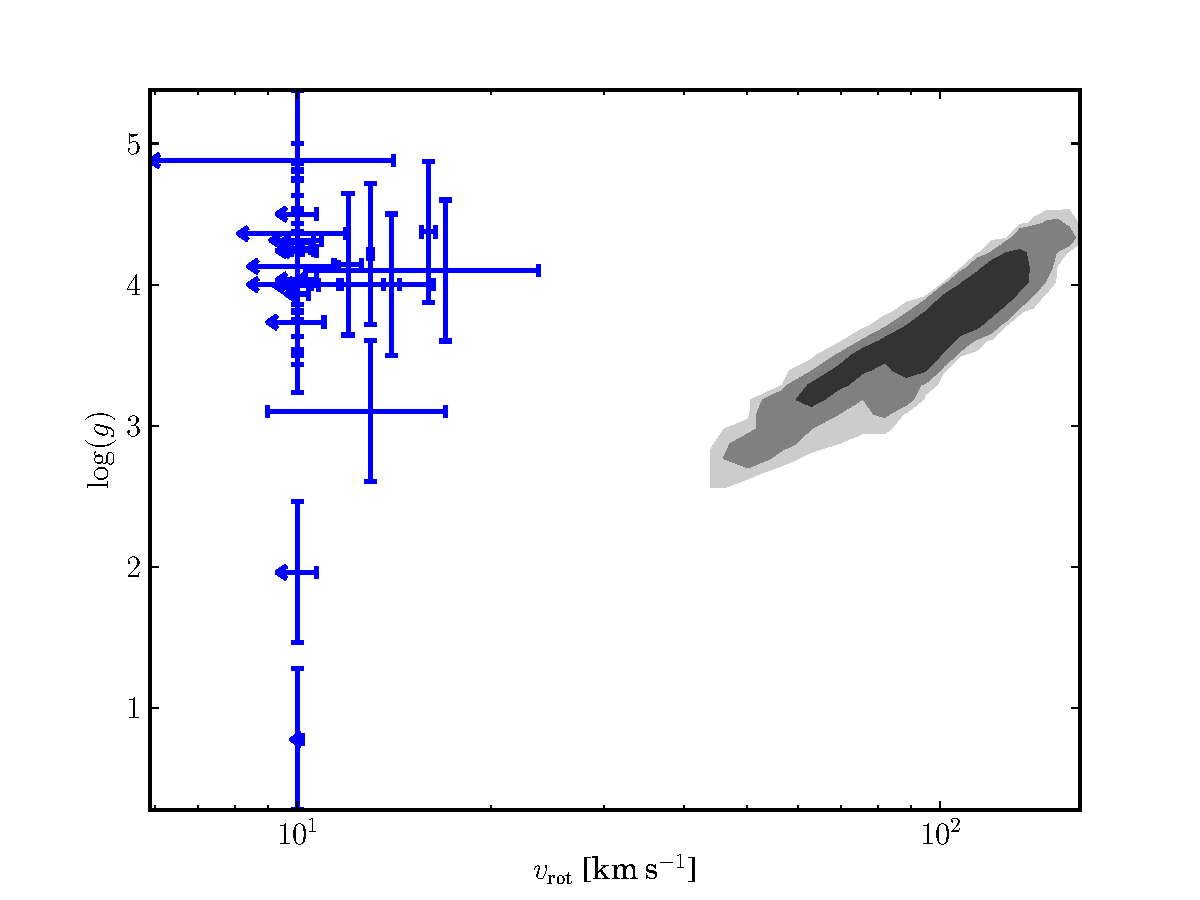
\includegraphics[width=\textwidth]{chapter_sn1006/plots/compare_vrot.pdf} 
   \caption[Comparison of rotation and surface gravity of SN 1006 candidates]{Comparison of the evolutionary state and rotational velocity of 55000 binary synthesis \glsentryname{sds} progenitors \citep[gray shades;data from][]{2008ApJ...677L.109H} with the measured rotation from this work. Due to the resolution of the spectrograph most of these stars only have an upper limit of the rotation speed of $\vrot=10~\kms$}
   \label{fig:han2008_vrot_compare}
\end{figure}


\begin{figure}[tb] %  figure placement: here, top, bottom, or page
   \centering
   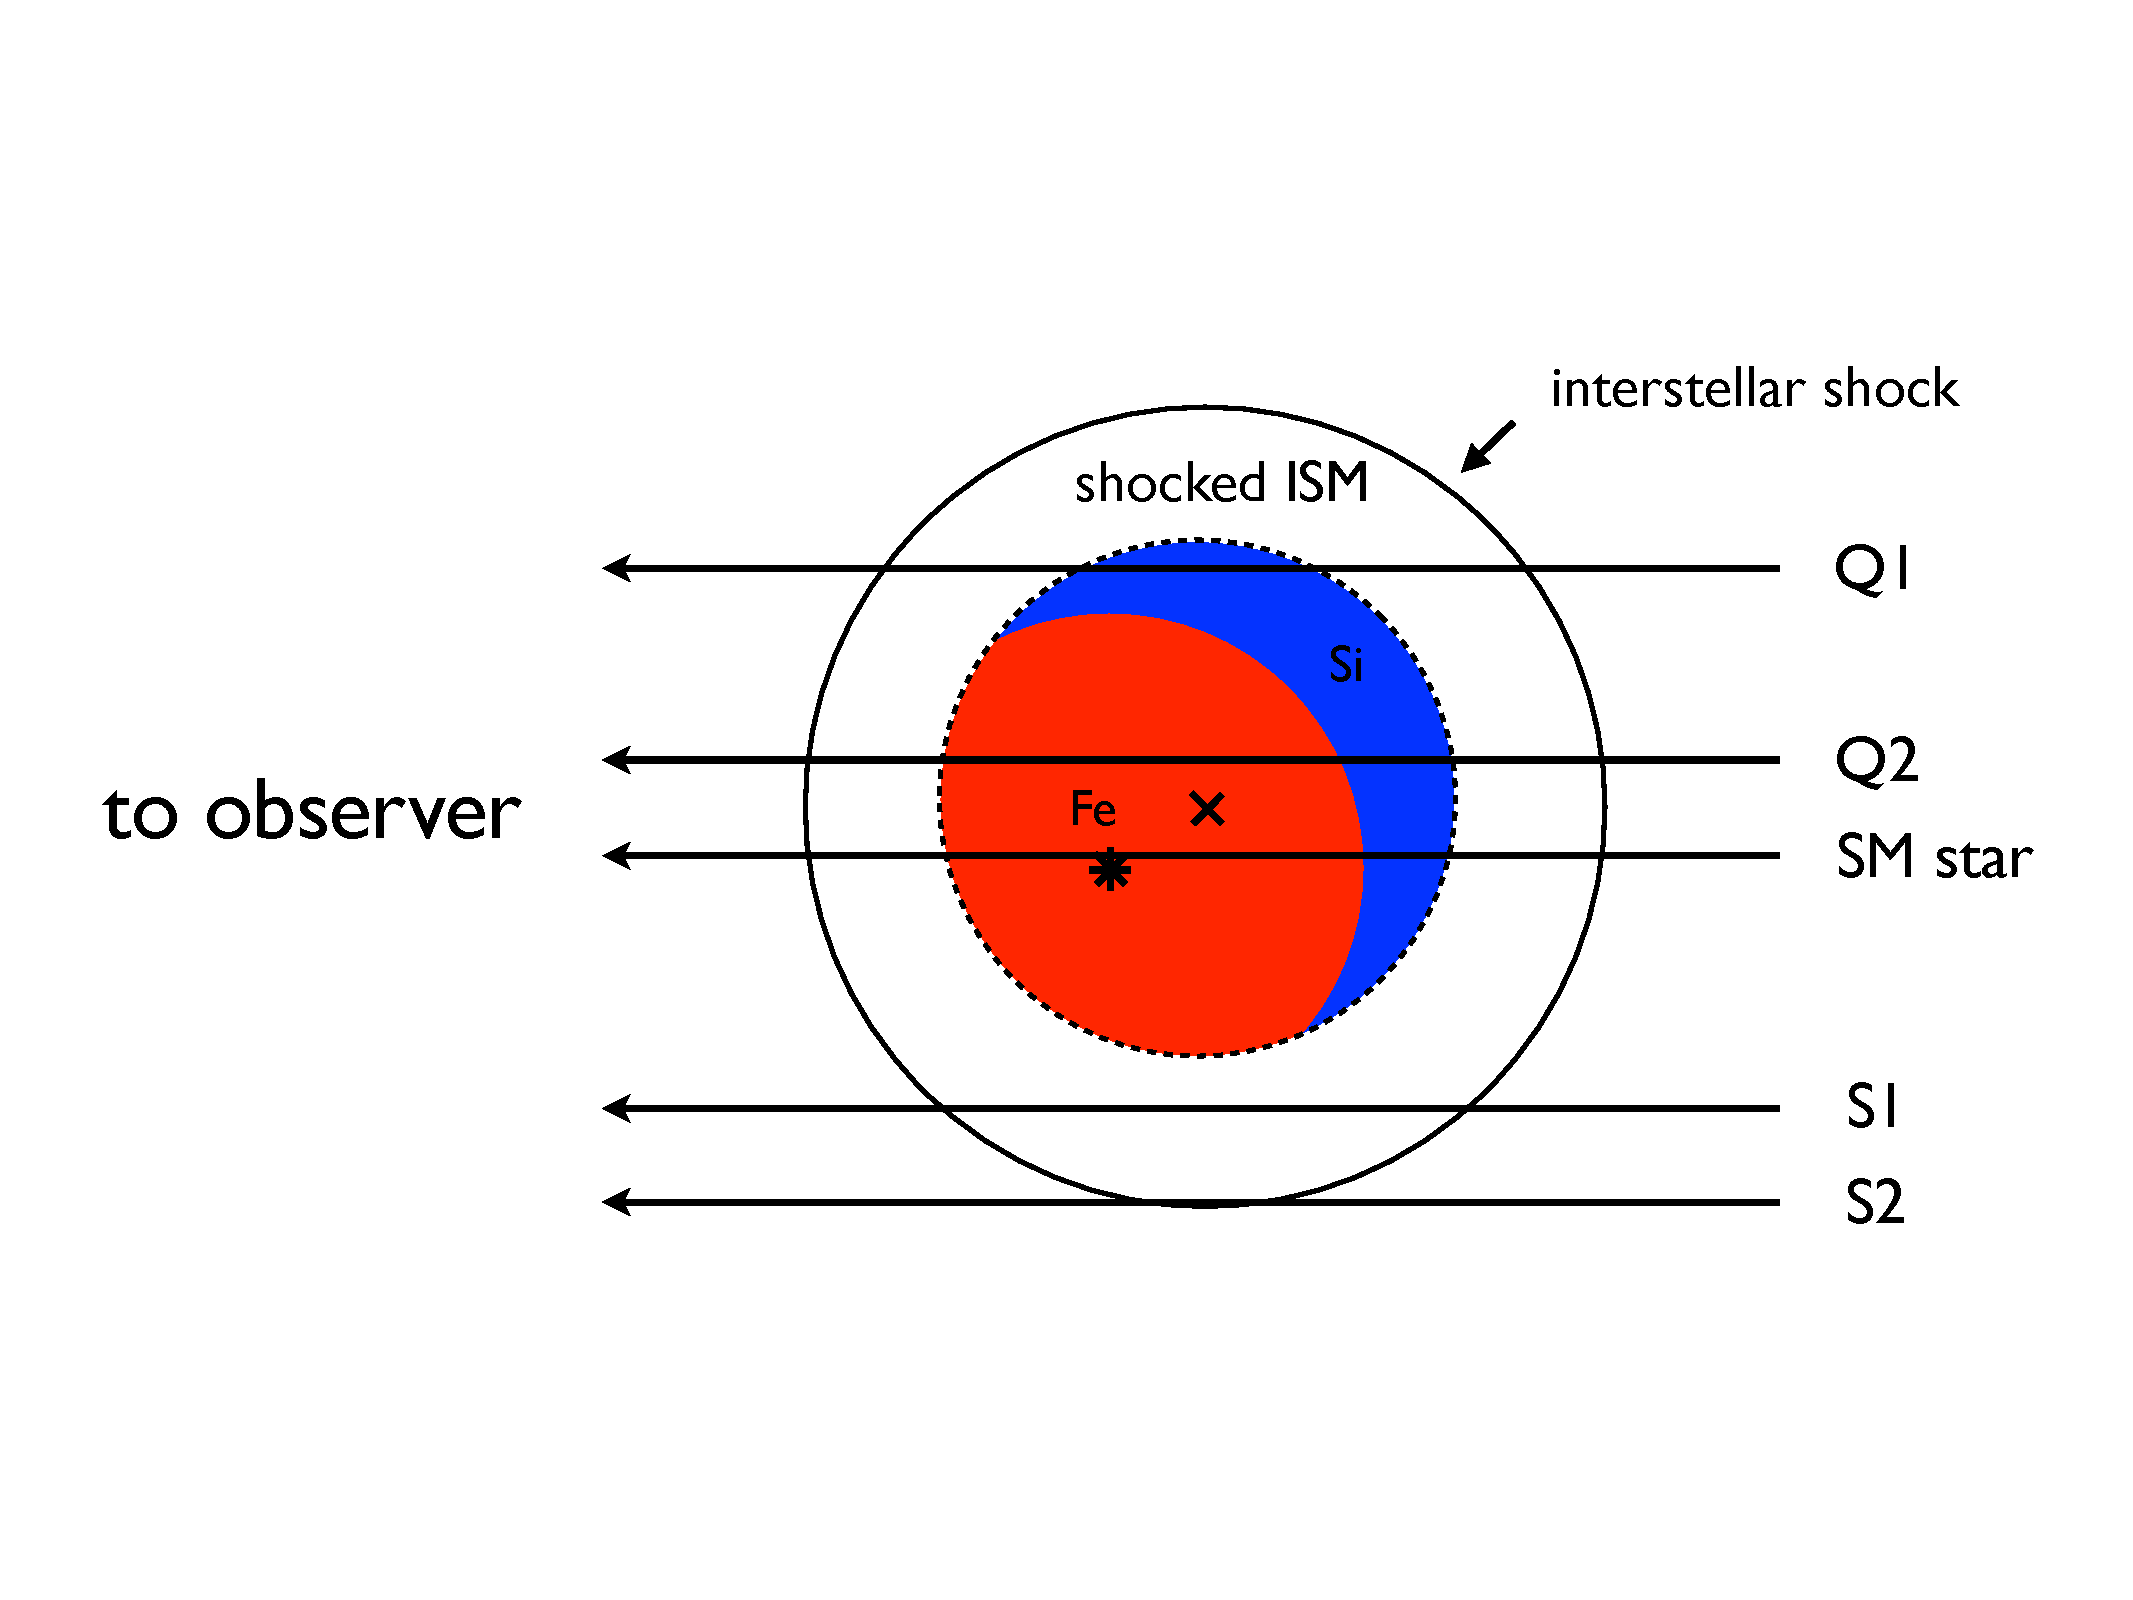
\includegraphics[width=\textwidth]{chapter_sn1006/plots/Winkler2005_probingsn1006_cropped.pdf} 
   \caption[Background UV sources probing the remnant]{Background UV sources probing the remnant. Figure adapted from \citet{2005ApJ...624..189W}}
   \label{fig:sn1006_uvprobe}
\end{figure}

The observations presented here for \sn{1006}{} are in conflict with the standard \snia\ donor star scenarios, which include accretion onto a white dwarf from a main sequence, sub giant, or giant companion. 
A few non-standard scenarios survive our observational tests. These include a helium white dwarf as a donor star (see Section \ref{sec:intro:subchandra}), which would not be detectable with our observations, although it is unlikely that a helium white dwarf would survive the explosion (priv. comm. R\"udiger Pakmor). The other possibility is that \sneia\ (or at least \sn{1006}{} and \sn{1572}{}) do not have donor stars, consistent with a \gls{dds}.

Another remnant that can be subjected to such an intensive search is Kepler (\sn{1604}). Kepler seems to be different from either \sn{1572}{} and \sn{1006}{}\ due to detection of interaction with the \gls{csm}. Observational facts of the Kepler remnant  as well as the description of the donor star search will be discussed in the conclusion of this thesis (Chapter \ref{chap:conclusion}).

